%TODO talk about 0.0 F1 score models
%TODO introduce the +/- 5% corridor in the first paragraph to disregard the insignificant results.
\section{Results}\label{ch:results}
During training, almost all $81$ trained models achieved a validation accuracy significantly above random guessing, except for the SRNN-2 models trained on the base and low LRD corpus, which scored $75.0\%$ and $50.4\%$ respectively. I have included them in the experiments regardless of their low validation accuracy, since it was unclear whether validation accuracy was a strong predictor for a network's performance on the experiment data. I present my results with regard to three focus points: First, the overall performance of different architectures with respect to which corpus they were trained on, then the individual model performances on each of the two experiments, and finally a closer look at classifications made by outlier networks - networks which drastically over- or underperformed in either of the experiments - with regards to word features.

\subsection{Architecture/Training Data}
\begin{table}[h]
\begin{tabularx}{\textwidth}{@{}l*{10}{C}c@{}}
 \toprule
  & \textit{Accuracy} &  \textit{Precision} &  \textit{Recall} &  \textit{F1 Score} &  \textit{Val Acc} \\
 \midrule
 SRNN & \multicolumn{5}{c}{Base} \\
 \midrule
	Mean & \textit{0.476} & \textit{0.278} & \textit{0.181} & \textit{0.193} & 0.972 \\
	Variance & 0.064 & 0.235 & 0.257 & 0.220 & 0.081 \\
 \midrule
 SRNN & \multicolumn{5}{c}{Low LRD} \\
 \midrule
	Mean & \textbf{0.514} & \textbf{0.443} & \textbf{0.288} & \textbf{0.316} & \textit{0.932} \\
	Variance & 0.055 & 0.176 & 0.259 & 0.213 & 0.158 \\
 \midrule
 SRNN & \multicolumn{5}{c}{High LRD} \\
 \midrule
	Mean & 0.511 & 0.415 & 0.153 & 0.200 & \textbf{0.981} \\
	Variance & 0.043 & 0.211 & 0.171 & 0.187 & 0.054 \\
 \midrule
 SRNN & \multicolumn{5}{c}{Complete} \\
 \midrule
	Mean & \textit{0.500} & 0.379 & \textbf{0.208} & \textbf{0.236} & \textit{0.962} \\
	Variance & 0.056 & 0.217 & 0.236 & 0.211 & 0.107 \\
 \midrule
 \midrule
 LSTM & \multicolumn{5}{c}{Base} \\
 \midrule
 Mean & \textbf{0.543} & \textit{0.219} & 0.148 & 0.154 & 0.999 \\
Variance & 0.173 & 0.365 & 0.335 & 0.341 & 0.003 \\
 \midrule
 LSTM & \multicolumn{5}{c}{Low LRD} \\
 \midrule
 Mean & 0.529 & \textbf{0.391} & \textbf{0.176} & \textbf{0.195} & 0.999 \\
Variance & 0.158 & 0.295 & 0.311 & 0.302 & 0.002 \\
 \midrule
 LSTM & \multicolumn{5}{c}{High LRD} \\
 \midrule
 Mean & \textit{0.472} & 0.258 & \textit{0.036} & \textit{0.059} & \textbf{1.000} \\
Variance & 0.075 & 0.278 & 0.057 & 0.090 & 0.000 \\
 \midrule
 LSTM & \multicolumn{5}{c}{Complete} \\
 \midrule
Mean & 0.515 & \textit{0.289} & \textit{0.120} & \textit{0.136} & \textbf{0.999} \\
Variance & 0.143 & 0.318 & 0.268 & 0.269 & 0.002 \\
 \midrule
 \midrule
 GRU & \multicolumn{5}{c}{Base} \\
 \midrule
 Mean & 0.531 & \textit{0.371} & 0.147 & 0.185 & 0.999 \\
Variance & 0.097 & 0.297 & 0.226 & 0.247 & 0.001 \\
 \midrule
 GRU & \multicolumn{5}{c}{Low LRD} \\
 \midrule
 Mean & \textbf{0.554} & \textbf{0.507} & \textbf{0.206} & \textbf{0.243} & 0.999 \\
Variance & 0.133 & 0.198 & 0.302 & 0.285 & 0.001 \\
 \midrule
 GRU & \multicolumn{5}{c}{High LRD} \\
 \midrule
 Mean & \textit{0.514} & 0.439 & \textit{0.126} & \textit{0.170} & \textit{0.972} \\
Variance & 0.082 & 0.223 & 0.198 & 0.193 & 0.055 \\
 \midrule
 GRU & \multicolumn{5}{c}{Complete} \\
 \midrule
Mean & \textbf{0.533} & \textbf{0.439} & 0.160 & 0.200 & 0.990 \\
Variance & 0.106 & 0.245 & 0.244 & 0.242 & 0.034 \\
\bottomrule
\end{tabularx}
\caption[Performance measures regardless of training corpus]{Performance measures of all architectures across both experiments depending on which corpus they were trained on, as well as the compounded measures for all networks regardless of training data.}
\label{tab:perf_all}
\end{table}
As can be seen in Table \ref{tab:perf_all}, none of the architectures consistently achieved an accuracy far above the random guessing baseline of $50.0\%$. However, there was still a notable difference in performance between architectures: on average, the GRU networks scored the highest on accuracy and precision, while the SRNN networks achieved the best recall and F1 score. With $51.5\%$, LSTMs scored an average accuracy between SRNNs ($50.0\%$) and GRUs ($53.3\%$), but they underperformed in all other experiment measures.

Furthermore, the choice of training data had a notable effect on overall model performance: SRNNs and GRUs received a boost in performance in all measures when comparing the Base to the Low LRD models, elevating SRNNs from an accuracy below random guessing to $51.4\%$. While LSTMs lost $1.4\%$ in terms of accuracy, all other performance measures improved significantly for the Low LRD models. Training on the High LRD corpus aided SRNNs in terms of accuracy, precision and F1 score, but worsened accuracy, recall and F1 score for LSTMs and GRUs.

\subsection{Experiment 1: Long-Range Dependency}\label{resultsLRD}
I report results for Experiment 1 in Tables \ref{tab:perf_LRDbase}, \ref{tab:perf_LRDlow} and \ref{tab:perf_LRDhigh}, which include the performance measures for all networks trained on the Base, Low and High LRD corpus respectively, as evaluated on Experiment 1.

\begin{table}[t]
\begin{tabularx}{\textwidth}{@{}l*{10}{C}c@{}}
\toprule
  \textit{Network} &  \textit{Accuracy} &  \textit{Precision} &  \textit{Recall} &  \textit{F1 Score} &  \textit{Val Acc} \\
\midrule
    GRU-2 &     0.890 &      \textbf{0.982} &   0.794 &     0.878 &    0.995 \\
    GRU-4 &     0.487 &      0.413 &   0.060 &     0.105 &    1.000 \\
    GRU-8 &     0.488 &      0.331 &   0.023 &     0.043 &    1.000 \\
   GRU-16 &     0.550 &      0.713 &   0.168 &     0.272 &    1.000 \\
   GRU-32 &     0.434 &      0.267 &   0.075 &     0.118 &    1.000 \\
   GRU-64 &     0.510 &      0.537 &   0.149 &     0.234 &    1.000 \\
  GRU-128 &     0.553 &      0.611 &   0.293 &     0.396 &    0.999 \\
  GRU-256 &     0.497 &      0.364 &   0.009 &     0.018 &    1.000 \\
  GRU-512 &     0.500 &      0.487 &   0.007 &     0.015 &    1.000 \\
   LSTM-2 &     0.500 &      0.000 &   0.000 &     0.000 &    0.999 \\
   LSTM-4 &     0.451 &      0.000 &   0.000 &     0.000 &    1.000 \\
   LSTM-8 &     \textbf{0.910} &      0.959 &   \textbf{0.857} &     \textbf{0.905} &    \textbf{1.000} \\
  LSTM-16 &     0.343 &      0.001 &   0.000 &     0.000 &    1.000 \\
  LSTM-32 &     0.500 &      0.000 &   0.000 &     0.000 &    1.000 \\
  LSTM-64 &     0.505 &      0.596 &   0.030 &     0.057 &    1.000 \\
 LSTM-128 &     0.347 &      0.001 &   0.000 &     0.000 &    1.000 \\
 LSTM-256 &     0.455 &      0.128 &   0.016 &     0.028 &    1.000 \\
 LSTM-512 &     0.499 &      0.468 &   0.009 &     0.017 &    0.991 \\
   SRNN-2 &     $0.465$ &      0.357 &   0.087 &     0.140 &    \textit{0.750} \\
   SRNN-4 &     $0.488$ &      0.334 &   0.023 &     0.043 &    1.000 \\
   SRNN-8 &     $0.461$ &      0.037 &   0.003 &     0.006 &    1.000 \\
  SRNN-16 &     $\textit{0.272}$ &      0.021 &   0.010 &     0.014 &    1.000 \\
  SRNN-32 &     0.498 &      0.492 &   0.141 &     0.219 &    1.000 \\
  SRNN-64 &     0.504 &      0.505 &   0.366 &     0.424 &    1.000 \\
 SRNN-128 &     0.484 &      0.040 &   0.001 &     0.003 &    1.000 \\
 SRNN-256 &     0.503 &      0.503 &   0.455 &     0.478 &    1.000 \\
 SRNN-512 &     0.484 &      0.017 &   0.001 &     0.001 &    1.000 \\
 \midrule
 \midrule
 \textbf{Mean} & 0.503 & 0.339 & 0.132 & 0.163 & 0.990 \\
 \textbf{Variance} & 0.130 & 0.294 & 0.233 & 0.253 & 0.048 \\
\bottomrule
\end{tabularx}
\caption[Base LRD trained network performance on experiment 1]{Performance measures for experiment 1 of all networks that were trained on the Base LRD corpus.}
\label{tab:perf_LRDbase}
\end{table}

When trained on the Base corpus, $8$ of $27$ models ($29.6\%$) achieved an accuracy above random guessing. Among those $8$, only $2$ reached an accuracy above $60\%$: LSTM-8 and GRU-2. The vast majority of models - $20$ in total - reached an accuracy of $50 \pm 5\%$. $4$ performed even worse than that: the worst model (SRNN-16) only achieved $27.2\%$ accuracy on the experiment data. There was no apparent correlation between validation accuracy and model performance in Experiment 1 - indeed, SRNN-2 with the lowest validation accuracy at $75.0\%$ evaluated at below chance, but so did several models with a validation accuracy of $100\%$.

\begin{table}
\begin{tabularx}{\textwidth}{@{}l*{10}{C}c@{}}
\toprule
  \textit{Network} &  \textit{Accuracy} &  \textit{Precision} &  \textit{Recall} &  \textit{F1 Score} &  \textit{Val Acc} \\
\midrule
    GRU-2 &     0.583 &      0.582 &   0.589 &     0.585 &    1.000 \\
    GRU-4 &     0.505 &      0.518 &   0.135 &     0.214 &    1.000 \\
    GRU-8 &     0.498 &      0.491 &   0.106 &     0.175 &    0.997 \\
   GRU-16 &     0.503 &      0.528 &   0.060 &     0.107 &    1.000 \\
   GRU-32 &     0.505 &      0.525 &   0.100 &     0.168 &    1.000 \\
   GRU-64 &     \textbf{0.890} &      \textbf{0.869} &   \textbf{0.918} &     \textbf{0.893} &    \textbf{1.000} \\
  GRU-128 &     0.484 &      0.324 &   0.030 &     0.054 &    1.000 \\
  GRU-256 &     0.500 &      0.496 &   0.039 &     0.072 &    1.000 \\
  GRU-512 &     0.500 &      0.435 &   0.002 &     0.004 &    0.997 \\
   LSTM-2 &     0.500 &      0.500 &   0.475 &     0.487 &    0.996 \\
   LSTM-4 &     \textit{0.278} &      \textit{0.000} &   \textit{0.000} &     \textit{0.000} &    \textit{1.000} \\
   LSTM-8 &     0.500 &      0.000 &   0.000 &     0.000 &    1.000 \\
  LSTM-16 &     0.881 &      0.853 &   0.920 &     0.885 &    1.000 \\
  LSTM-32 &     0.491 &      0.092 &   0.002 &     0.004 &    1.000 \\
  LSTM-64 &     0.500 &      0.505 &   0.010 &     0.020 &    1.000 \\
 LSTM-128 &     0.496 &      0.374 &   0.011 &     0.021 &    0.998 \\
 LSTM-256 &     0.500 &      0.535 &   0.007 &     0.014 &    1.000 \\
 LSTM-512 &     0.507 &      0.566 &   0.058 &     0.106 &    1.000 \\
   SRNN-2 &     0.501 &      0.501 &   0.366 &     0.423 &    0.\textit{504} \\
   SRNN-4 &     0.708 &      0.646 &   0.922 &     0.760 &    0.930 \\
   SRNN-8 &     0.508 &      0.527 &   0.150 &     0.234 &    1.000 \\
  SRNN-16 &     0.500 &      0.000 &   0.000 &     0.000 &    1.000 \\
  SRNN-32 &     0.486 &      0.388 &   0.050 &     0.088 &    1.000 \\
  SRNN-64 &     0.487 &      0.375 &   0.040 &     0.072 &    1.000 \\
 SRNN-128 &     0.492 &      0.484 &   0.236 &     0.318 &    0.953 \\
 SRNN-256 &     0.501 &      0.501 &   0.412 &     0.452 &    1.000 \\
 SRNN-512 &     0.503 &      0.503 &   0.497 &     0.500 &    1.000 \\
 \midrule
 \midrule
 \textbf{Mean} & 0.530 & 0.449 & 0.227 & 0.246 & 0.977 \\
 \textbf{Variance} & 0.120 & 0.217 & 0.304 & 0.280 & 0.096 \\
\bottomrule
\end{tabularx}
\caption[Low LRD trained network performance on experiment 1]{Performance measures for experiment 1 of all networks that were trained on the Low LRD corpus.}
\label{tab:perf_LRDlow}
\end{table}

$12$ of $27$ Low LRD-trained models ($44.4\%$) scored an accuracy higher than the random guessing baseline. Among those, $3$ models - SRNN-4, LSTM-16 and GRU-64 - reached an accuracy above $60\%$. While $22$ models fell within the $50 \pm 5\%$ belt of accuracy, only $1$ model performed significantly worse: LSTM-4 with $27.8\%$. Validation accuracy was entirely unrelated to model performance, with LSTM-4 having achieved a perfect score on the validation data, but completely failing at Experiment 1. On average, all measures have improved when compared to the Base models: accuracy improved by $+2.7$ percentage points (p.p.), precision by $+11.0$ p.p., recall by $+9.5$ p.p. and F1 score by $+8.3$ p.p.

\begin{table}
\begin{tabularx}{\textwidth}{@{}l*{10}{C}c@{}}
 \toprule
  \textit{Network} &  \textit{Accuracy} &  \textit{Precision} &  \textit{Recall} &  \textit{F1 Score} &  \textit{Val Acc} \\
 \midrule
    GRU-2 &     0.494 &      0.480 &   0.136 &     0.212 &    1.000 \\
    GRU-4 &     0.499 &      0.482 &   0.036 &     0.066 &    1.000 \\
    GRU-8 &     0.342 &      0.000 &   0.000 &     0.000 &    1.000 \\
   GRU-16 &     0.523 &      0.590 &   0.153 &     0.242 &    1.000 \\
   GRU-32 &     0.504 &      0.521 &   0.093 &     0.158 &    1.000 \\
   GRU-64 &     0.504 &      0.522 &   0.088 &     0.150 &    1.000 \\
  GRU-128 &     0.489 &      0.419 &   0.056 &     0.098 &    1.000 \\
  GRU-256 &     0.503 &      0.549 &   0.035 &     0.066 &    0.902 \\
  GRU-512 &     \textbf{0.800} &      \textbf{0.768} &   \textbf{0.861} &     \textbf{0.812} &    0.849 \\
   LSTM-2 &     0.483 &      0.390 &   0.060 &     0.104 &    1.000 \\
   LSTM-4 &     \textit{0.282} &      \textit{0.000} &   \textit{0.000} &     \textit{0.000} &    1.000 \\
   LSTM-8 &     0.379 &      0.000 &   0.000 &     0.000 &    1.000 \\
  LSTM-16 &     0.502 &      0.640 &   0.007 &     0.015 &    1.000 \\
  LSTM-32 &     0.498 &      0.475 &   0.038 &     0.070 &    1.000 \\
  LSTM-64 &     0.500 &      0.000 &   0.000 &     0.000 &    1.000 \\
 LSTM-128 &     0.492 &      0.365 &   0.022 &     0.041 &    1.000 \\
 LSTM-256 &     0.497 &      0.367 &   0.008 &     0.016 &    1.000 \\
 LSTM-512 &     0.500 &      0.000 &   0.000 &     0.000 &    0.999 \\
   SRNN-2 &     0.500 &      0.499 &   0.042 &     0.078 &    \textit{0.833} \\
   SRNN-4 &     0.502 &      0.523 &   0.046 &     0.085 &    0.996 \\
   SRNN-8 &     0.539 &      0.622 &   0.201 &     0.304 &    1.000 \\
  SRNN-16 &     0.500 &      0.000 &   0.000 &     0.000 &    0.999 \\
  SRNN-32 &     0.500 &      0.497 &   0.037 &     0.070 &    1.000 \\
  SRNN-64 &     0.503 &      0.504 &   0.360 &     0.420 &    1.000 \\
 SRNN-128 &     0.497 &      0.494 &   0.235 &     0.318 &    1.000 \\
 SRNN-256 &     0.496 &      0.495 &   0.340 &     0.403 &    1.000 \\
 SRNN-512 &     0.490 &      0.459 &   0.112 &     0.180 &    1.000 \\
 \midrule
 \midrule
 \textbf{Mean} & 0.493 & 0.395 & 0.110 & 0.145 & 0.984 \\
 \textbf{Variance} & 0.083 & 0.230 & 0.180 & 0.182 & 0.045 \\
 \bottomrule
\end{tabularx}
\caption[High LRD trained network performance on experiment 1]{Performance measures for experiment 1 of all networks that were trained on the high LRD corpus.}
\label{tab:perf_LRDhigh}
\end{table}

$9$ of $27$ High LRD-trained models ($33.3\%$) achieved an accuracy above baseline, but only GRU-512 by a significant margin with $80\%$. $23$ models performed within the $\pm 5\%$ margin around the baseline, and $3$ models (LSTM-4, LSTM-8 and GRU-8) underperfomed significantly. There was no relation between validation accuracy and performance on experiment data for High LRD models, either. Compared to the Base models, High LRD models almost consistently scored worse: accuracy, recall and F1 score went down by $-1.0$, $-2.2$ and $-1.8$ p.p. respectively, but precision was improved by $+5.6$ p.p.

\subsection{Experiment 2: New Depths}\label{resultsND}
All results for Experiment 2 can be found in Tables \ref{tab:perf_NDbase}, \ref{tab:perf_NDlow} and \ref{tab:perf_NDhigh}. When comparing mean performances across all models, they largely scored higher on Experiment 2 than Experiment 1. This suggests that Experiment 2 was easier regardless of training data. As with Experiment 1, a model's validation accuracy did not correlate with its performance on the experiment data.

\begin{tabular}{lrrrrr}
\toprule
  network &  accuracy &  precision &  recall &  f1\_score &  val\_acc \\
\midrule
    GRU-2 &     0.500 &      0.000 &   0.000 &     0.000 &    0.995 \\
    GRU-4 &     0.563 &      0.655 &   0.265 &     0.377 &    1.000 \\
    GRU-8 &     0.472 &      0.164 &   0.014 &     0.025 &    1.000 \\
   GRU-16 &     0.500 &      0.000 &   0.000 &     0.000 &    1.000 \\
   GRU-32 &     0.500 &      0.000 &   0.000 &     0.000 &    1.000 \\
   GRU-64 &     0.515 &      0.550 &   0.160 &     0.248 &    1.000 \\
  GRU-128 &     0.496 &      0.000 &   0.000 &     0.000 &    0.999 \\
  GRU-256 &     0.500 &      0.000 &   0.000 &     0.000 &    1.000 \\
  GRU-512 &     0.601 &      0.597 &   0.620 &     0.608 &    1.000 \\
   LSTM-2 &     0.500 &      0.000 &   0.000 &     0.000 &    0.999 \\
   LSTM-4 &     0.500 &      0.000 &   0.000 &     0.000 &    1.000 \\
   LSTM-8 &     0.500 &      0.000 &   0.000 &     0.000 &    1.000 \\
  LSTM-16 &     0.500 &      0.000 &   0.000 &     0.000 &    1.000 \\
  LSTM-32 &     0.778 &      0.792 &   0.755 &     0.773 &    1.000 \\
  LSTM-64 &     0.500 &      0.000 &   0.000 &     0.000 &    1.000 \\
 LSTM-128 &     0.993 &      0.991 &   0.995 &     0.993 &    1.000 \\
 LSTM-256 &     0.500 &      0.000 &   0.000 &     0.000 &    1.000 \\
 LSTM-512 &     0.499 &      0.000 &   0.000 &     0.000 &    0.991 \\
   SRNN-2 &     0.580 &      0.548 &   0.917 &     0.686 &    0.750 \\
   SRNN-4 &     0.488 &      0.000 &   0.000 &     0.000 &    1.000 \\
   SRNN-8 &     0.500 &      0.000 &   0.000 &     0.000 &    1.000 \\
  SRNN-16 &     0.500 &      0.000 &   0.000 &     0.000 &    1.000 \\
  SRNN-32 &     0.515 &      0.564 &   0.136 &     0.220 &    1.000 \\
  SRNN-64 &     0.511 &      0.529 &   0.192 &     0.281 &    1.000 \\
 SRNN-128 &     0.441 &      0.409 &   0.266 &     0.322 &    1.000 \\
 SRNN-256 &     0.382 &      0.156 &   0.053 &     0.080 &    1.000 \\
 SRNN-512 &     0.497 &      0.497 &   0.615 &     0.550 &    1.000 \\
\bottomrule
\end{tabular}


Among the Base models, $8$ of $27$ ($29.6\%$) performed above guessing baseline in Experiment 2 - the same ratio as for Experiment 1, though there was minimal overlap in the best performers. Only GRU-64 and SRNN-64 performed above $50\%$ accuracy for both experiments. $20$ of $27$ models stayed in the $\pm 5\%$ margin of the baseline, with only $2$ (SRNN-128 and SRNN-256) dropping below that. The best performing network - LSTM-128 - scored the highest accuracy across all models and all experiments with $99.3\%$.

\begin{table}
\begin{tabularx}{\textwidth}{@{}l*{10}{C}c@{}}
\toprule
  \textit{Network} &  \textit{Accuracy} &  \textit{Precision} &  \textit{Recall} &  \textit{F1 Score} &  \textit{Val Acc} \\
\midrule
    GRU-2 &     0.494 &      0.488 &   0.222 &     0.306 &    1.000 \\
    GRU-4 &     0.561 &      0.651 &   0.262 &     0.374 &    1.000 \\
    GRU-8 &     0.499 &      0.492 &   0.056 &     0.101 &    0.997 \\
   GRU-16 &     0.497 &      0.465 &   0.039 &     0.072 &    1.000 \\
   GRU-32 &     0.500 &      0.000 &   0.000 &     0.000 &    1.000 \\
   GRU-64 &     0.935 &      0.910 &   0.966 &     0.937 &    1.000 \\
  GRU-128 &     0.516 &      0.560 &   0.144 &     0.229 &    1.000 \\
  GRU-256 &     0.499 &      0.486 &   0.043 &     0.078 &    1.000 \\
  GRU-512 &     0.497 &      0.305 &   0.004 &     0.008 &    0.997 \\
   LSTM-2 &     0.499 &      0.000 &   0.000 &     0.000 &    0.996 \\
   LSTM-4 &     0.480 &      0.328 &   0.037 &     0.067 &    1.000 \\
   LSTM-8 &     0.555 &      0.660 &   0.226 &     0.337 &    1.000 \\
  LSTM-16 &     0.566 &      0.662 &   0.270 &     0.384 &    1.000 \\
  LSTM-32 &     \textit{0.327} &      0.207 &   0.122 &     0.154 &    1.000 \\
  LSTM-64 &     0.491 &      0.301 &   0.014 &     0.026 &    1.000 \\
 LSTM-128 &     0.500 &      0.000 &   0.000 &     0.000 &    0.998 \\
 LSTM-256 &     0.502 &      0.538 &   0.027 &     0.051 &    1.000 \\
 LSTM-512 &     \textbf{0.953} &      \textbf{0.917} &   \textbf{0.996} &     \textbf{0.955} &    \textbf{1.000} \\
   SRNN-2 &     0.501 &      0.501 &   0.585 &     0.540 &    \textit{0.504} \\
   SRNN-4 &     0.442 &      0.361 &   0.149 &     0.211 &    0.930 \\
   SRNN-8 &     0.529 &      0.582 &   0.206 &     0.304 &    1.000 \\
  SRNN-16 &     0.498 &      0.000 &   0.000 &     0.000 &    1.000 \\
  SRNN-32 &     0.580 &      0.561 &   0.738 &     0.637 &    1.000 \\
  SRNN-64 &     0.514 &      0.546 &   0.170 &     0.260 &    1.000 \\
 SRNN-128 &     0.498 &      0.495 &   0.178 &     0.262 &    0.953 \\
 SRNN-256 &     0.500 &      0.499 &   0.348 &     0.410 &    1.000 \\
 SRNN-512 &     0.501 &      0.505 &   0.136 &     0.214 &    1.000 \\
 \midrule
 \midrule
 \textbf{Mean} & 0.535 & 0.445 & 0.220 & 0.256 & 0.977 \\
 \textbf{Variance} & 0.126 & 0.246 & 0.281 & 0.263 & 0.096 \\
\bottomrule
\end{tabularx}
\caption[Low LRD trained network performance on experiment 2]{Performance measures for experiment 2 of all networks that were trained on the Low LRD corpus.}
\label{tab:perf_NDlow}
\end{table}

The same number of Low LRD models performed above chance for Experiment 2 as for Experiment 1 ($44.4\%$), with $6$ models (SRNN-2, SRNN-8, LSTM-16, LSTM-512, GRU-4 and GRU-64) occuring in both groups. LSTM-512 and GRU-64 have both achieved an accuracy $>90\%$. $19$ models performed within the $\pm 5\%$ margin around the baseline, only $2$ dropped below that. Compared to the Base models, low LRD models also performed better on Experiment 2: mean accuracy is up by $+0.4$ p.p., precision by $+20.6$, recall by $+3.5$ and F1 score by $6.5$ p.p.

\begin{table}
\begin{tabularx}{\textwidth}{@{}l*{10}{C}c@{}}
\toprule
  \textit{Network} &  \textit{Accuracy} &  \textit{Precision} &  \textit{Recall} &  \textit{F1 Score} &  \textit{Val Acc} \\
\midrule
    GRU-2 &     0.535 &      0.580 &   0.253 &     0.353 &    1.000 \\
    GRU-4 &     0.502 &      0.518 &   0.070 &     0.123 &    1.000 \\
    GRU-8 &     0.500 &      0.000 &   0.000 &     0.000 &    1.000 \\
   GRU-16 &     0.492 &      0.269 &   0.010 &     0.019 &    1.000 \\
   GRU-32 &     0.511 &      0.552 &   0.114 &     0.189 &    1.000 \\
   GRU-64 &     0.502 &      0.512 &   0.081 &     0.140 &    1.000 \\
  GRU-128 &     0.541 &      0.601 &   0.244 &     0.347 &    1.000 \\
  GRU-256 &     0.503 &      0.530 &   0.048 &     0.089 &    0.902 \\
  GRU-512 &     0.500 &      0.000 &   0.000 &     0.000 &    0.849 \\
   LSTM-2 &     0.531 &      0.591 &   0.200 &     0.299 &    1.000 \\
   LSTM-4 &     0.500 &      0.000 &   0.000 &     0.000 &    1.000 \\
   LSTM-8 &     0.500 &      0.000 &   0.000 &     0.000 &    1.000 \\
  LSTM-16 &     0.517 &      0.658 &   0.070 &     0.127 &    1.000 \\
  LSTM-32 &     0.511 &      0.554 &   0.112 &     0.187 &    1.000 \\
  LSTM-64 &     \textit{0.285} &      0.000 &   0.000 &     0.000 &    1.000 \\
 LSTM-128 &     0.500 &      0.000 &   0.000 &     0.000 &    1.000 \\
 LSTM-256 &     0.521 &      0.608 &   0.121 &     0.202 &    1.000 \\
 LSTM-512 &     0.500 &      0.000 &   0.000 &     0.000 &    0.999 \\
   SRNN-2 &     0.491 &      0.333 &   0.017 &     0.033 &    \textit{0.833} \\
   SRNN-4 &     0.500 &      0.000 &   0.000 &     0.000 &    0.996 \\
   SRNN-8 &     0.500 &      0.000 &   0.000 &     0.000 &    1.000 \\
  SRNN-16 &     \textbf{0.675} &      \textbf{0.691} &   \textbf{0.633} &     \textbf{0.661} &    0.999 \\
  SRNN-32 &     0.507 &      0.557 &   0.072 &     0.128 &    1.000 \\
  SRNN-64 &     0.492 &      0.473 &   0.139 &     0.215 &    1.000 \\
 SRNN-128 &     0.485 &      0.281 &   0.019 &     0.036 &    1.000 \\
 SRNN-256 &     0.501 &      0.502 &   0.322 &     0.392 &    1.000 \\
 SRNN-512 &     0.512 &      0.534 &   0.183 &     0.273 &    1.000 \\
 \midrule
 \midrule
 \textbf{Mean} & 0.504 & 0.346 & 0.100 & 0.141 & 0.984 \\
 \textbf{Variance} & 0.056 & 0.267 & 0.141 & 0.164 & 0.045 \\
\bottomrule
\end{tabularx}
\caption[High LRD trained network performance on experiment 2]{Performance measures for experiment 2 of all networks that were trained on the High LRD corpus.}
\label{tab:perf_NDhigh}
\end{table}
While the highest number of High LRD models have achieved an accuracy above random guessing - $10$ of $27$, or $37.0\%$ - only SRNN-16 crossed the $60\%$ threshold at all. Indeed, aside from SRNN-16, only one other model lay outside of the $\pm 5\%$ margin around the baseline - LSTM-64, with an accuracy of $28.5\%$. When comparing with the Base models, all measures except for precision, which improved by $+10.7$ p.p. Accuracy went down by $-2.7$ p.p., recall by $-7.5$ and F1 score by $-5.0$ p.p.

\subsection{Outliers: A Closer Look}
As is evident from the results described so far, a vast majority of models fell within a $\pm 5\%$ margin around random guessing in terms of accuracy. I consider these models to not have extracted any useful grammar information from the training data and discard them for further investigation. As such, I will only discuss models with an accuracy either $> 55\%$ or $< 45\%$, to both gather information on what caused models to succeed, and what caused them to fail.

First, I report the number of the two error categories (superfluous open bracket, superfluous closed bracket) per network architecture in Table ???. Hypothetically, since both categories were balanced in training and experiment data, there should be no significant difference between misclassifying one or the other - unless one category proves to be more complex to an architecture. The ratio of open-to-closed bracket misclassifications serves as a simple indication of whether the model extracted the correct information - that the amount of brackets needs to be balanced throughout a valid word - at all. A ratio of $1$ implies no model difference between the two categories. Conversely, any skewing above or below $1$ shows the model disproportionally struggling with one of the two categories.
%TODO table
%TODO which models skew from a ratio of 1?
%TODO is there predominant skewing?

To investigate properties of wrongly classified words, I scrutinize false positives for two word properties. I chose the properties as proxy values for word complexity: the maximum nesting depth of the word, and the position of the error within the word. Since all words within an experiment have the same length, variation in complexity can only arise through structural differences - like a deeper underlying parse tree. The values were averaged across all model instances with the same architecture and training corpus for reasons of simplicity, i.e. the results of both good base GRU outliers in Experiment 1 were merged. A low value in mean error position means that the model tended to misclassify words where the error occured early on in the word, while a high value means that the error occured later. Maximum nesting depth is an overall measure of complexity for the word, and refers to the deepest nesting level within the word. It is unrelated to the error position. Again, a low value means that the model predominantly misclassified words with a low nesting depth.



\begin{figure}[!tbp]
	\begin{minipage}{\textwidth}
     \centering
     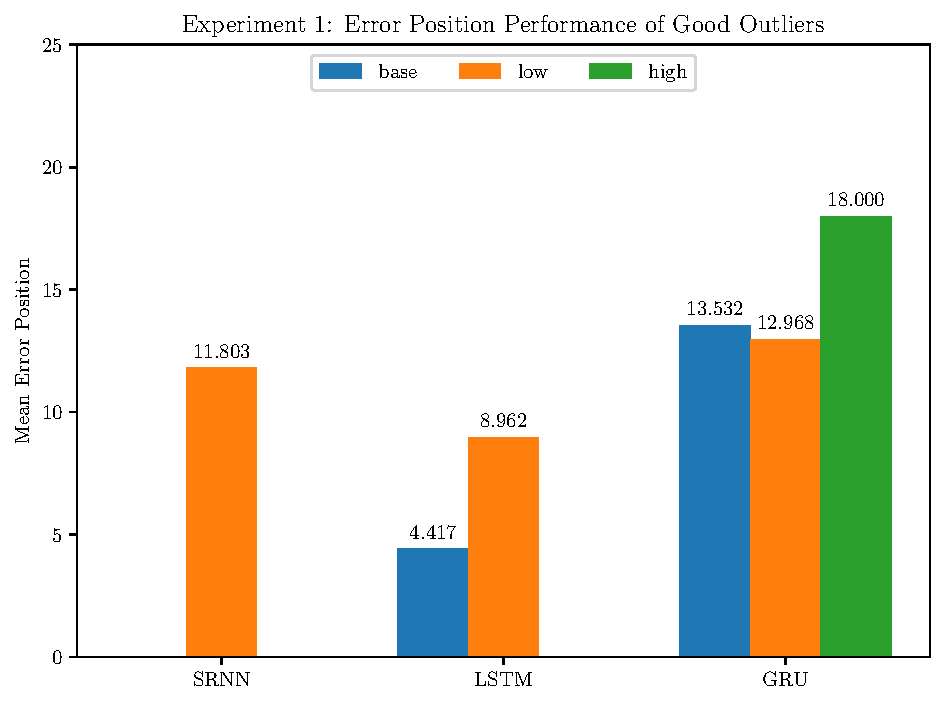
\includegraphics[width=.45\textwidth]{fig/LRD_error_pos_good}\quad
     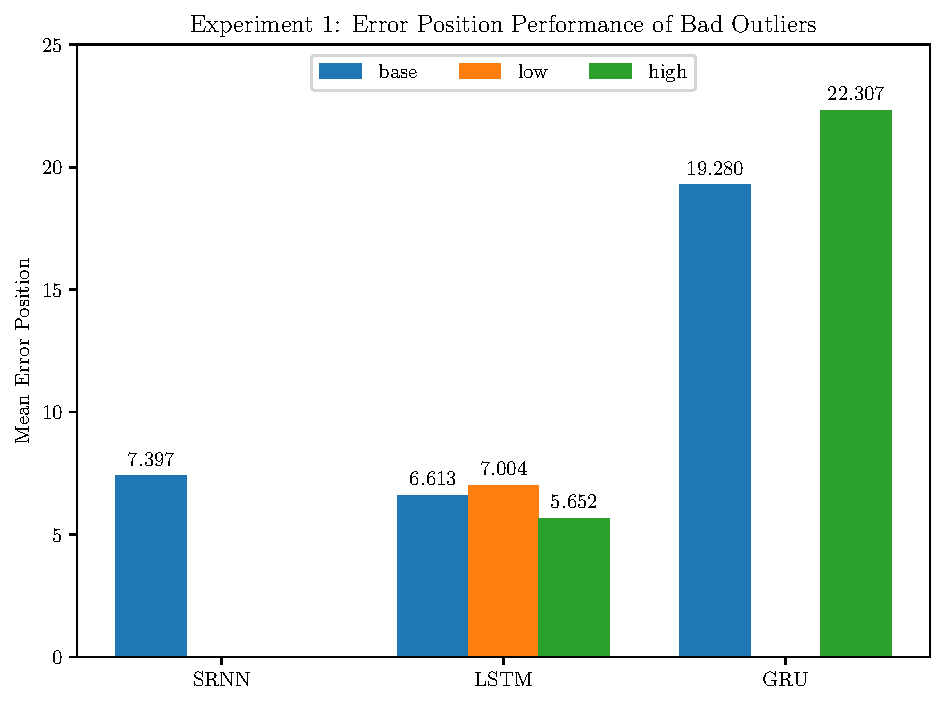
\includegraphics[width=.45\textwidth]{fig/LRD_error_pos_bad}\\
     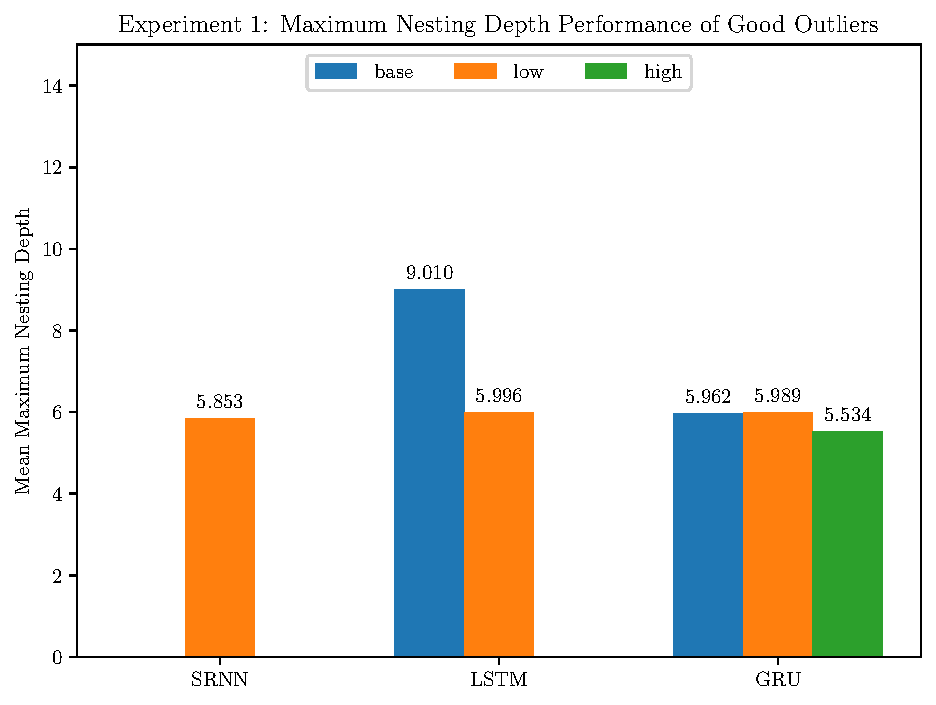
\includegraphics[width=.45\textwidth]{fig/LRD_max_valid_nesting_depth_good}\quad
     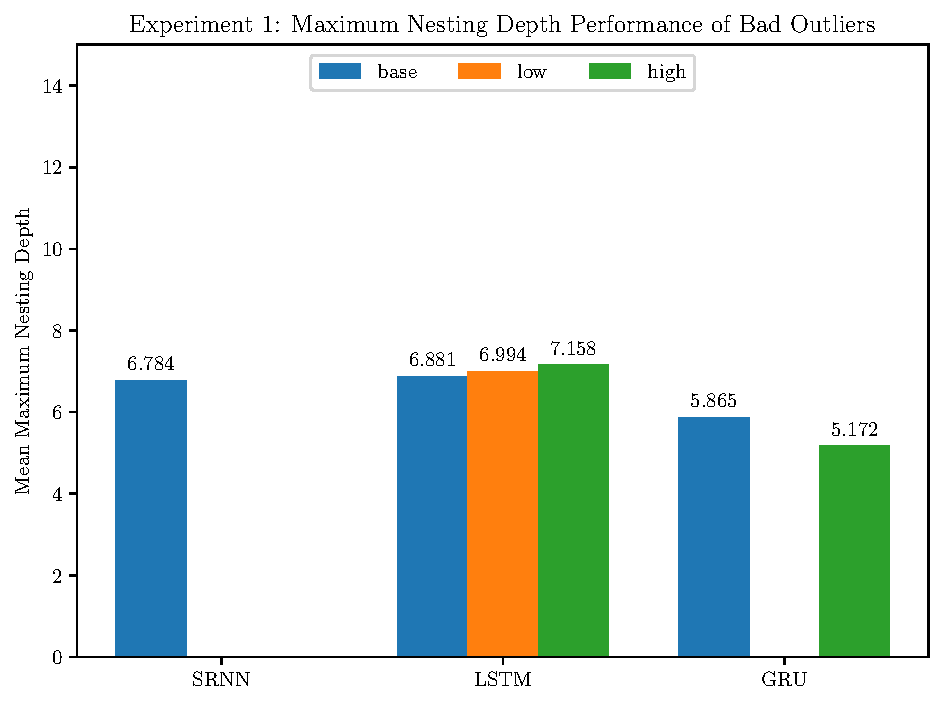
\includegraphics[width=.45\textwidth]{fig/LRD_max_valid_nesting_depth_bad}
     \subcaption{Properties of false positives in Experiment 1.}
     \label{fig:FP_Prop_LRD}
   \end{minipage}\\[1em]
   \begin{minipage}{\textwidth}
     \centering
     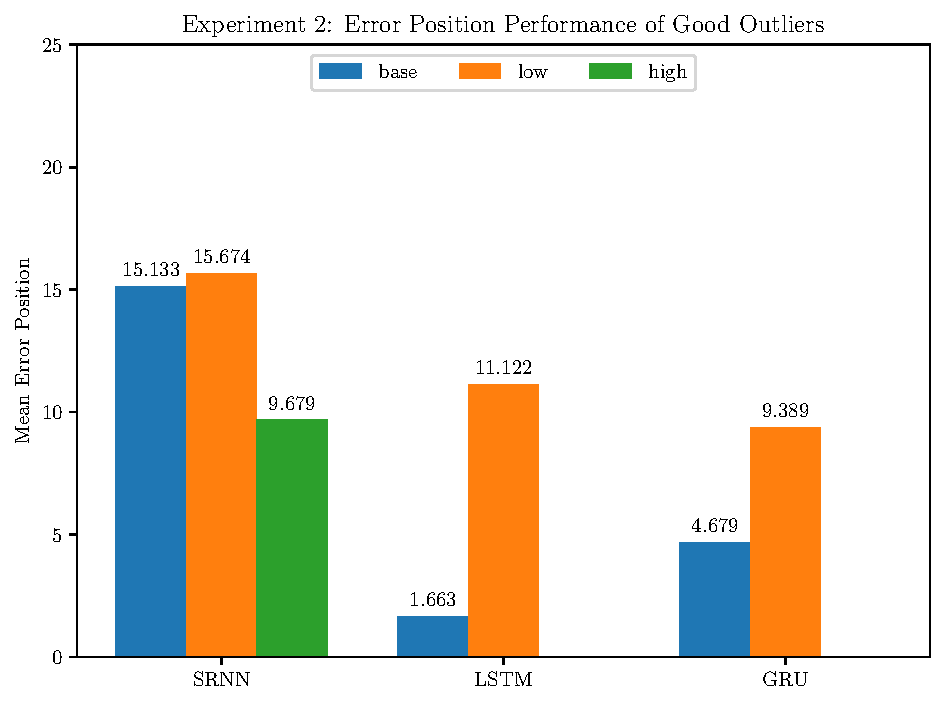
\includegraphics[width=.45\textwidth]{fig/ND_error_pos_good}\quad
     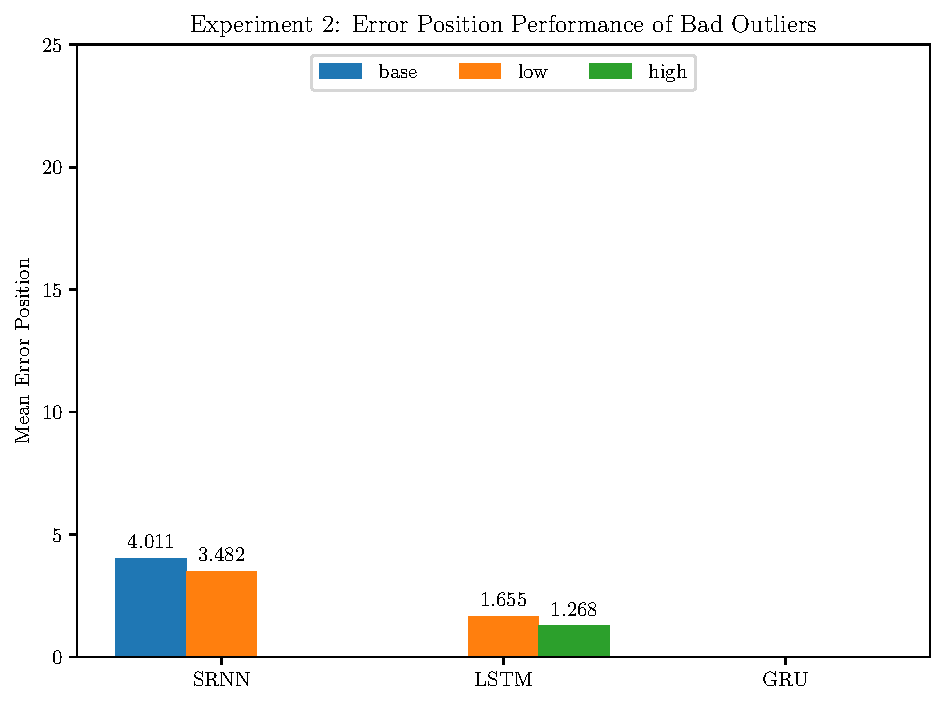
\includegraphics[width=.45\textwidth]{fig/ND_error_pos_bad}\\
     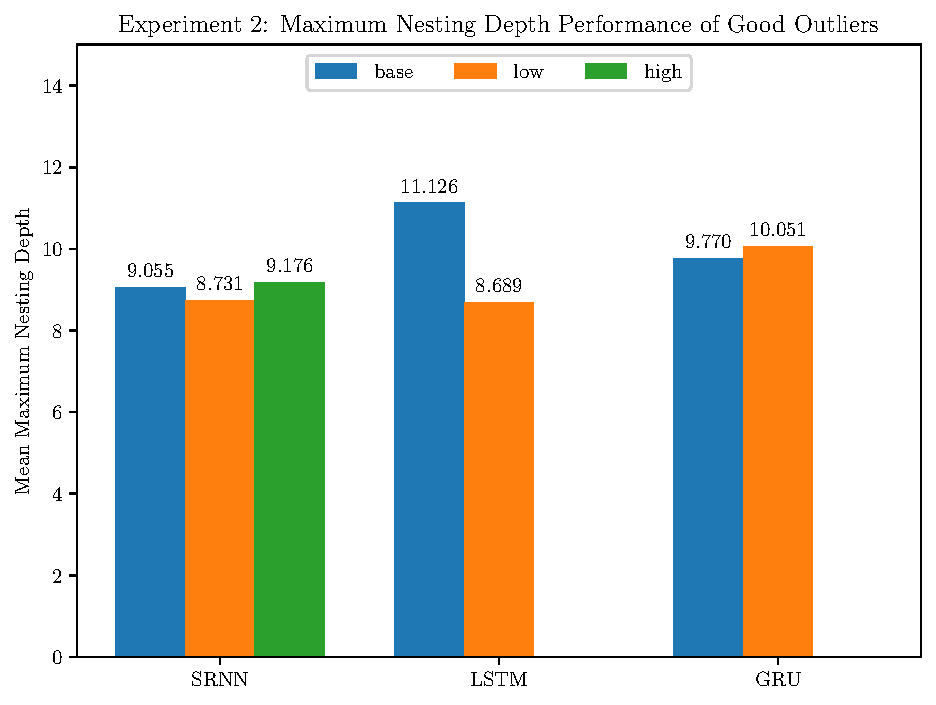
\includegraphics[width=.45\textwidth]{fig/ND_max_valid_nesting_depth_good}\quad
     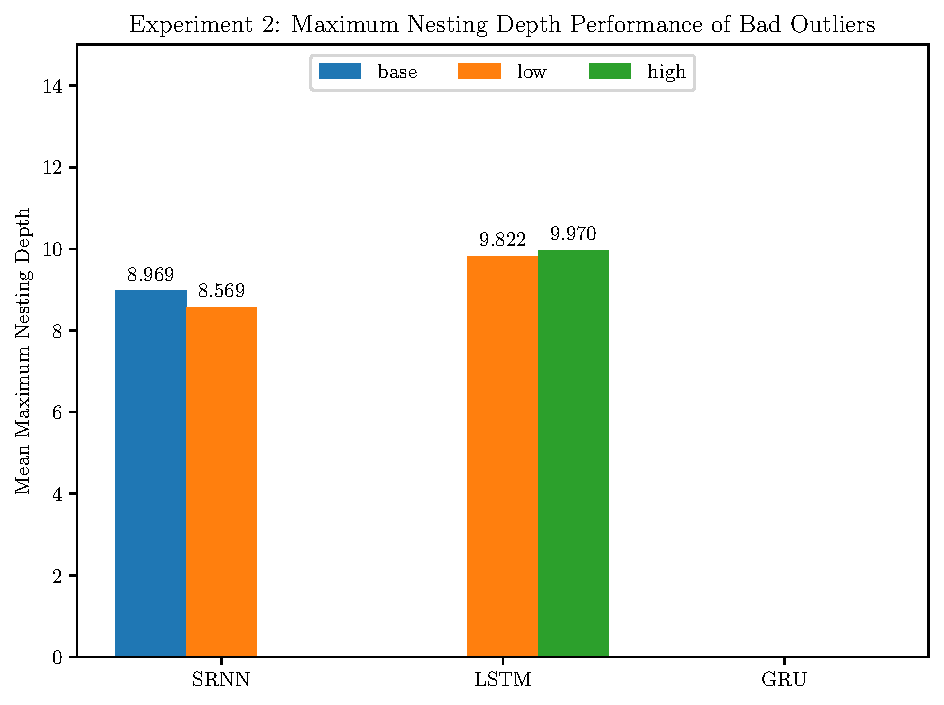
\includegraphics[width=.45\textwidth]{fig/ND_max_valid_nesting_depth_bad}
     \subcaption{Properties of false positives in Experiment 2.}
     \label{fig:FP_Prop_ND}
   \end{minipage}\\
  \caption{Properties of false positives as classified by different architectures.}
\end{figure}

% THIS GOES IN DISCUSSION
%While all these words were misclassified, a strong effect of word complexity still implies that the models process the linear input in a structural manner. They may not have learned an accurate representation of $D_{2}$, but they are likely to have learned a structured approximation.
%TODO